%introduction
In this section we would like to analyse the main differences between the \textit{AXI interconnect} of the Cortex M3 example design and the \textit{AXI connect}, the module which we had implemented.
In particular, the first paragraph explains how the signals pass through the two AXI and the delays given by them, while the second focuses on some post-synthesis features of our communication component.

{\color{Blue}{\subsection{Time Differences}}}

Comparing the two implementation and the simulations it is possible to notice that the handshake protocol provided by our configuration is faster than that achieved by the other.
This is because, whereas we design a set of multiplexers and demultiplexers to make the connection among master and slaves, the AXI of the example is composed by three main type of components:

{\flushleft
\begin{description}

\item[Slave Coupler:]Used as interface for the Cortex M3, it converts the \textbf{AXI3 protocol} of the processor to the \textbf{AXI4-lite protocol} of \textit{Xbar} and the peripherals. As a consequence, this conversion introduces a delay into the main signal of both write and read operations (In our implementation the conversion is provided by the component \textit{AXI4lite adapter} which hides a simple wire connection for only the signals used).

\item[Xbar:]The most interesting element of \textit{AXI interconnect} its main function is to initialize and manage the communication between a \textit{Slave Coupler} and a \textit{Master Coupler}. Therefore, the delay introduced by it is not only for choosing the right master interface to associate but also to achieve the handshake protocol among the interfaces (in our implementation the handshake protocol is managed by the master and slave themselves).
The Figure \ref{RWXbar} shows an example of read and write operations of the \textit{Xbar}.

\item[Master Coupler:]Like the \textit{Slave Coupler} but without conversion logic, it is used as interface for peripheral.

\end{description}
}

For more information about the \textit{AXI interconnection} and its components, see \cite{AXIInterconnectGuide}.

\begin{figure}[!hb]
  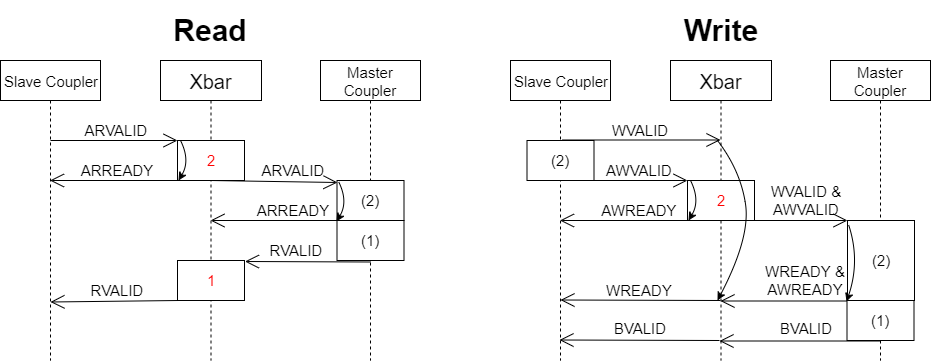
\includegraphics[width=\textwidth]{./../../img/Images/Read_Write_xbar}
  \caption{Read and write communication on Xbar with {\color{Red}Xbar delays} and other latencies (curly arrow to identify the communication's sections)}
  \label{RWXbar}
\end{figure}



{\color{Blue}{\subsection{Signal Propagation}}}
Our implementation is safer but more costly
